 \documentclass[journal]{IEEEtran}
\interdisplaylinepenalty=2500

\usepackage{array}
\usepackage{graphicx}
\usepackage{epsf}
\usepackage{float}
\usepackage{stfloats}
\usepackage[font=footnotesize]{caption}
\usepackage[font=footnotesize]{subcaption}
\usepackage{cite}
\usepackage{picinpar}
\usepackage{siunitx}

\usepackage{amsmath, nccmath}
\usepackage{url}
\usepackage{flushend}
\usepackage{colortbl}
\usepackage{soul}
\usepackage{multirow}
\usepackage{pifont}
\usepackage{color}
\usepackage{alltt}
\usepackage[hidelinks]{hyperref}
\usepackage{enumerate}
\usepackage{siunitx}
\usepackage{breakurl}
\usepackage{epstopdf}
\usepackage{pbox}


\usepackage{booktabs}
\usepackage{wrapfig}

\graphicspath{{../}}

\usepackage{placeins}
\usepackage{latexsym}
\usepackage{amssymb}
\usepackage{xifthen}
\usepackage{balance}
\usepackage{multicol}
\renewcommand{\arraystretch}{1.2}




\newenvironment{conditions}
  {\par\vspace{\abovedisplayskip}\noindent\begin{tabular}{>{$}l<{$} @{${}-{}$} l}}
  {\end{tabular}\par\vspace{\belowdisplayskip}}


\ifCLASSINFOpdf

\else
 
\fi


\hyphenation{op-tical net-works semi-conduc-tor}


\begin{document}

\title{Analysis and DSP Implementation of Multisampled Three-Phase Current Controller}


% make the title area
\maketitle

\begin{abstract}
nothing yet
\end{abstract}

% Note that keywords are not normally used for peerreview papers.
\begin{IEEEkeywords}
nothing yet
\end{IEEEkeywords}


\IEEEpeerreviewmaketitle

\section{Introduction}
\IEEEPARstart{F}{ield} oriented control (FOC) in electrical drives and voltage oriented control (VOC) in grid-connected converters is a well-established strategy for the control of high performance three-phase electrical systems \cite{holmes2012}. An essential part of this concept is the inner current control loop \cite{holmes2009}. A prerequisite for the proper operation of the outer control loops is a precise and rapid digital current controller ~\cite{yepes2014,choi1998}. Robustness at high output frequencies, along with a decoupled d and q axis transient operation is very important for high-speed electrical drives ~\cite{choi1998,hoffmann2016,yim2009}. Digital control introduces delays due to the sampling process, execution time and digital pulse width modulation (DPWM) \cite{holmes2009}. These delays limit the achievable bandwidths and motivate the direct discrete-time domain design of high-performance current controllers \cite{bae2003}. 
In most state-of-the-art applications, double-sampled double-update (DS-DU-PWM) control strategy is used, where the inductor currents are sampled twice per PWM period, with acquisition instants synchronized to obtain average current value. In industrial applications, feedback signal is often strongly corrupted by various noise sources, which requires additional filtering of the signal []. This is well-achieved by oversampling the signal and then averaging it over PWM period. In this way, true-average is obtained with additional high noise suppression. After oversampling and filtering the signal, decimation to double-update is used for perfoming the control algorithm. This kind of strategy is labeled as multi-sampled double-update (MS-DU-PWM) control. The MS-DU-PWM strategy leads to a high quality feedback signal, however, with great impact on the system dynamics. 
The delay-related limitations have inspired investigating multisampled PWM control, with purpose of enabling analog-like control bandwidths in digital systems. The multisampled multi-update (MS-MU-PWM) approach relies on acquiring the control variables and updating the modulating waveform multiple times per switching period \cite{corradini_analysis}. The concept of MS-MU-PWM digital control offers significant reduction of control and modulator delays and therefore is a promising solution for breaking the bandwidth limitations \cite{corradini2018}. [jos gomila citata za multisamping electrical drives]. On the other hand, MS-MU-PWM introduces a set of nonlinearities due to sampling of the switching ripple, which is why certain digital filtering should always be present [petric2021]. Most of the nonlinearities are strongly attenuated filtering the switching ripple, for example using moving average filters (MAFs).

Synchronous rotating frame (SRF) PI controllers are the most frequently encountered current control strategies for three-phase $RL$ loads due to their simplicity and satisfactory performance for the majority of the industry requirements ~\cite{rowan1986,bae2003,yepes2014}. With a proper parameter setting procedure, high bandwidths can be achieved ~\cite{yepes2014,holmes2009}. Nevertheless, their transient decoupling capability is rather limited, especially at high speeds \cite{lorenz2000}. On the other hand, model predictive dead-beat current controllers offer very fast transient response but at the cost of considerable performance degradation when parameter mismatch occurs ~\cite{malesani1999,xu2019} [DB MS citati]. Since saturation and temperature variations are very often encountered in electrical drives, a simple dead-beat approach might lead to insufficient performance. An FPGA implementation of the robust multisampled dead-beat control has been proposed in \cite{rovere2018}. Another often-implemented current control strategy is the discrete internal model principle (IMC) design \cite{lorenz2010}. Since no S domain based delay approximations are used, axes cross-coupling is inherently eliminated and high closed loop bandwidths can be achieved at very high operating frequencies ~\cite{commentsHoffmann,vuksa2016} [petric IMC salient].

This paper analyzes the use of the discrete IMC based current controller with MS-MU-PWM, suitable for implementation on standard DSP platforms. The main goal of the paper is to analyze the performance of MS-MU-PWM in standard industrial applications, and to compare it with standardly used DS-DU-PWM and MS-DU-PWM methods. 
%The MS-PWM control strategy is analyzed for three different control loop organizations. The first one uses discrete IMC controller from \cite{vuksa2016}, with a moving average filter (MAF) in the feedback. This case is found to offer slightly improved dynamics compared to standard use of double-update with the same discrete IMC (without filter in feedback) ~\cite{lorenz2010,vuksa2016}, with significant improvement in jitter suppression. Due to added delays introduced by the MAF, the second case adds a derivative action to the controller structure, as in \cite{vuksa2016}. This case is given to demonstrate that MS-PWM can offer even better dynamics than reported in \cite{vuksa2016}. The final case implements MS-PWM based discrete IMC, without any filters in feedback. This case is expected to provide the best dynamics, using discrete IMC without derivative gain. The feedback quality is expected to worsen compared to cases with MAFs, hower, it still retains higher quality compared to double-update \cite{petric2020}. 
The target is to show that the MS-MU-PWM control can offer high quality feedback signal as in MS-DU-PWM, obtained by averaging over switching period, while also providing improved dynamic capabilities compared to DS-DU-PWM. With modern processors indeed offering more and more computational power, implementing MS-MU-PWM with feedback averaging has a potential of becoming the standard industrial procedure for digital control.

%This paper is organized as follows. Section II addresses discrete time machine model, controller structure and analyzes delays introduced by feedback averaging, calculation and DPWM. The multisampling PWM approach, with an outline of its merits and demerits, is explained in Section III. A DSP implementation of the multisampling algorithm is also presented. Exact controller structures and parameter setting procedures for the three aforementioned cases of interest are derived in Section IV. Effectiveness of the derived analytical model is illustrated via simulated current loop step responses and frequency response analyses. Comparison between performance of the proposed methodology and benchmark controllers is also provided. Experimental results are shown in section V. Conclusions are drawn in section VI, along with a proposal for further studies on the presented topic.
 
\section{Multi-rate control system}

\begin{figure*}[t!]
    \centerline{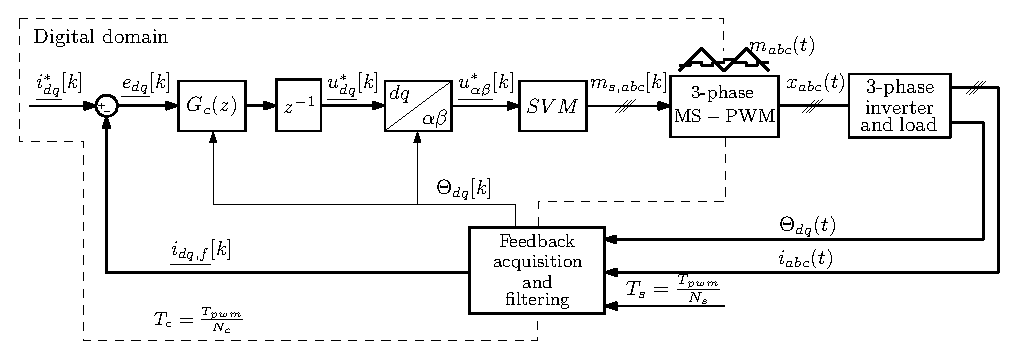
\includegraphics[width=0.95\linewidth]{figures/schematic.eps}}
    \caption{Multisampled control loop of a three-phase inverter. ubaci 1/z da bi bio kompatibilan sa tajming dijagramom. Takodje, ubaci Feedback acquisition park transform and filtering}
    \label{fig:MSControl}
\end{figure*}

The multi-rate control system of a three-phase $RL$ load in $dq$ frame is shown in Fig. 1. The system can be separated into digital and continuous-time domain. An ADC is used to transform feedback signal from analog to digital domain. This action is performed with a sampling frequency $f_s = N_s f_{pwm}$, where $N_s$ is the oversampling factor and $f_{pwm}$ is the switching frequency of the inverter. The digital domain operates with frequency $f_c = N_c f_{pwm}$, where $N_c$ is the multi-update factor that determines the update rate of the controller output. The choice of this frequency is independent of the sampling frequency, as the feedback signal can be oversampled with frequency $f_s$ and then filtered and decimated to control frequency $f_c$. The digital domain is comprised of feedback filter $G_{fb}(z)$, controller $G_c(z)$, coordinate frame transformation block, and modulation block. The controller $G_c(z)$ outputs reference voltage in $dq$ frame, $\underline{u_{dq}}^*[k]$, which is then transformed to $\alpha \beta$ frame. This reference voltage is used to obtain digital modulating waveform for each inverter phase, $m_s,{abc}[k]$. Conversion from digital to analog domain is performed by MS-PWM. Its inherent zero-order hold function transforms the digital impulse train $m_{s,abc}[k]$ into the continuous-time modulating waveform $m_{abc}(t)$. Due to favourable characteristics in multi-update applications, MS-PWM with the triangular carrier is used. The PWM output is used as a gate signal $x_{abc}(t)$. The three-phase inverter is used to supply the $RL$ load, which can be a three-phase machine or electrical grid. The sensed feedback includes line currents $i_{\alpha \beta}(t)$ and the angle of the $dq$ coordinate frame $\Theta_{dq}$. 

\subsection{Motivation behind multisampling}

Modern processors feature high computational power, which enables short execution times for control routines. However, switching frequencies of the converter are still hardware limited, and do not go over several tens of kHz for industrial drive applications. This hardware based limitation directly affects the realizable bandwidths of the current control loop, which subsequently limits the speed and position responses as well. Therefore, using multisampled PWM control [] seems to be a logical step forward in the high-performance drive control. 
Using describing function approach, small-signal model of the multisampled PWM with triangular carrier is found to be almost equal to a pure delay of $\frac{T_c}{2}$, where $T_c$ is the modulating waveform update period []:

\begin{equation}
\begin{aligned}
G_{DPWM} (s) = \frac{d(s)}{m(s)} = A(\omega,D,N_c) e^{-s\frac{T_c}{2}},
\label{eq:DPWM} 
\end{aligned}    
\end{equation}
where $s$ is the complex variable of the Laplace transform, $d$ is the continuous-time duty cycle used for averaged modeling [], and $D$ is the steady-state duty cycle. The gain $A$ can be approximated with unity gain with negligible losses in modeling accuracy [].

In DSP applications, update of the modulating waveform is usually delayed by one control period $T_c$, due to the non-negligible computational time []. This results in total digital delays resulting from computation and PWM modulation being equal to:

\begin{equation}
\begin{aligned}
\tau_{d} = \frac{3}{2}T_c = \frac{3}{2} \frac{T_{pwm}}{N_c}
\label{eq:tauD} 
\end{aligned}    
\end{equation}

From this, it can be seen that multi-update control reduced digital delays inversely proportionate to the multi-update factor $N_c$. Traditionally, double-update is the most often used method, which results in twice decreased delays compared to single-update.
Term multisampled (multi-update) control is most often used when $N_c$ is increased above 2. This kind of control is a promising way of bringing the digital control close to analog regarding achievable bandwidths []. However, care must be taken as significant nonlinearities are also introduced in the control system, mainly due to the discontinuity of the modulating waveform, which now features switching ripple component as well. For this reason, multi-update control is most often followed by feedback filtering, which removes the switching ripple from the feedback signal []. 

\subsection{Discrete-time model of a three-phase RL load}

Given the simplicity of the inverter topology with a $RL$ load, its model can be easily derived directly in discrete-time domain, without the use of Tustin's method and transport delay approximations []. This kind of modeling is important for design of digital controllers, as it enables highest achievable bandwidths with inherent decoupling of $dq$ axes []. 
Note that for direct-discrete modeling, the action of the PWM is assumed to be equal to a zero-order hold in stationary $\alpha \beta$ frame []. This is true for the case of single- and double-update PWM, however, for $N_c>2$, the exact model is shown in \ref{eq:DPWM}. For the very specific case of triangular carrier, regarding its phase response, MS-PWM can still be approximated well, specially regarding its phase response, by a ZOH with update rate equal to $f_c$, which justifies this approximation necessary for the direct-discrete modeling.

The required discrete-time modeling can be found in [lorenz2010,vuksa2016,DOI 10.1109/TPEL.2018.2841206]. The methods in these papers feature different procedures, but the end model is unique. This paper follows the procedure from [DOI 10.1109/TPEL.2018.2841206].
In order to analyze the system as single-input single-output (SISO), complex variables are used []. 
Starting from $\alpha \beta$ frame differential equations necessary for modeling are:

\begin{equation}
\begin{aligned}
\underline{u}_{\alpha \beta} (t) = R \underline{i}_{\alpha \beta} (t) + L \frac{d}{dt} \underline{i}_{\alpha \beta} (t),
\label{eq:alphaBetaVoltage} 
\end{aligned}    
\end{equation}
where $R$ and $L$ are the line resistance and the line inductance, respectively. The three-phase $RL$ load usually also consists of a series voltage source, which models the machine back-emf or the grid voltage. It is neglected in this analysis, as the paper focuses purely on enhancing the current-loop response, without taking into account disturbance rejection.
The s-domain transfer function from applied voltage to the line current, corresponding to \ref{eq:alphaBetaVoltage} is:

\begin{equation}
\begin{aligned}
G_{i,\alpha \beta} = \frac{1}{R} \frac{1}{1 + s \frac{L}{R}}.
\label{eq:sDomainAlphaBeta} 
\end{aligned}    
\end{equation}


The one-step delay of the controller output update is represented as $e^{-s T_c}$. The PWM is modeled as a ZOH:

\begin{equation}
\begin{aligned}
G_{DPWM,\alpha \beta} \approx \frac{1-e^{-sT_c}}{s}.
\label{eq:DPWMAlphaBeta} 
\end{aligned}    
\end{equation}

The transformation from $\alpha \beta$ to $dq$ frame is obtained using the substitution $s \rightarrow s + j \omega_o$, where $\omega_o$ is the $dq$ frame rotating frequency.
This yields the following s-domain transfer function of the controlled plant in $dq$ frame:

\begin{equation}
\begin{aligned}
G_{p,dq}(s) = e^{-s T_c} e^{-j\omega_o} \frac{1-e^{-sT_c}e^{-j\omega_oT_c}}{s+j\omega_o} \frac{1}{R} \frac{1}{1 + s \frac{L}{R} + j\omega_o \frac{L}{R}}.
\label{eq:modelSdomain} 
\end{aligned}    
\end{equation}
 
The discrete-time model is obtained using $\mathcal{Z}$ transform table to transform \ref{eq:modelSdomain}:

\begin{equation}
\begin{aligned}
G_{p,dq}(z) = \frac{\left( 1 - e^{-\frac{R}{L}T_c}\right) e^{-2j\omega_o T_c}}{R} \frac{1}{z \left( z - e^{- \left( \frac{R}{L} + j\omega_o\right) T_c}\right)},
\label{eq:modelZdomain} 
\end{aligned}    
\end{equation}
where $z$ is the complex variable of the $\mathcal{Z}$ transform.

The model obtained in \ref{eq:modelZdomain} is used for the subsequent derivation of the model-based controller.
 
\subsection{Discrete IMC controller}


\begin{figure}[t!]
    \centerline{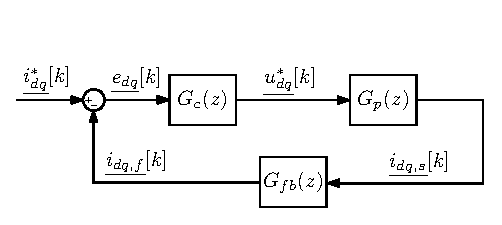
\includegraphics[width=0.95\linewidth]{figures/small_signal.eps}}
    \caption{Small-signal block diagram of the system from Fig. \ref{fig:MSControl} in discrete-time domain.}
    \label{fig:SmallSignal}
\end{figure}

The $dq$ frame discrete-time small signal representation of the control system in Fig. \ref{fig:MSControl} is shown in Fig. \ref{fig:SmallSignal}. In this paper, IMC method is used to obtain the controller structure []. The goal of the method is to inverse the plan model with addition of a integrator with gain $\alpha$ that determines the crossover frequency []. For the sake of causality, due to digital delays, additional factor of $\frac{1}{z^2}$ is added to the controller structure, which results in the following transfer function:

\begin{equation}
\begin{aligned}
G_{c}(z) = \alpha \frac{1}{z^2} G^{-1}_{p,dq}(z)  =  \alpha XXX,
\label{eq:Controller} 
\end{aligned}    
\end{equation}
where $XXX = xxx$.

By implementing controller from \eqref{eq:Controller}, without any feedback filters, open-loop transfer function is obtained:

\begin{equation}
\begin{aligned}
W_{ol,1}(z) = \alpha \frac{z}{z-1}
\label{eq:Controller} 
\end{aligned}    
\end{equation}

This kind of open-loop structure is the state-of-the-art when it comes to DS-DU-PWM methods, often used in industry. In [vuksa] it is shown that relying on two samples per $T_{pwm}$ often results in unacceptable feedback signal deterioration in industrial applications. This is due to the unalignement between the voltage impulse and sampling instants due to limited current sensor bandwidths, analog feedback filters, delays in driver circuits, ADC conversion time, etc. Furthermore, feedback signal often comprises oscillations due to the $LC$ parasitics of long cables that are often present in industrial drives. This is a motivation behind the implementation of MS-DU-PWM, and in this paper MS-MU-PWM methods, where the signal is highly oversampled and than averaged over $T_{pwm}$.

\section{Feedback acquisition, coordinate frame transformation, and filtering}

\subsection{Feedback acquisition and $\alpha \beta - dq$ transformation}

The timing diagram of feedback acquisition, frame transformation and controller update is shown in Fig. \ref{fig:timings}. The modulating waveform is illustrated for one phase, $m_a(t)$.
The system analyzed in this paper features two independent discrete-time frequencies. First one is the control frequency, which defines the controller execution rate and update of the modulating waveform. It is defined by the multi-update factor $f_c = N_c f_{pwm}$. Control interrupts are synchronized with the carrier $\omega(t)$ such that two are always occurring at instants when carrier is equal to its maximum and zero value. Fig. \ref{fig:timings} is given for $N_c = 4$. At instant $k$, $dq$ frame feedback current $i_{dq,f}[k]$ is obtained and used to calculate the voltage reference $u^*_{dq}[k]$, which is used to calculate the segment of the modulating waveform that is applied at the beginning of the following control interrupt. As reported in [], $N_c$ should be chosen as the highest possible value allowed by the DSP processing power, in order to decrease the MS-PWM nonlinearities introduced by the discontinuities of the modulating waveforms. The synchronous frame signal $\Theta_{dq}$ is obtained each $T_c$ by implementing a PLL or using resolver/encoder sensors. 
The second independent frequency is the sampling frequency, which is defined by the multisampling factor the multisampling factor $f_s = N_s f_{pwm}$. This factor allows the DSP to acquire the signal with much higher rate than it can calculate control algorithms, by employing standardly available DMA module. High sampling rates allow the subsequent use of digital filters, most often moving average filters (MAFs), to obtain better quality feedback signal, after which the filtered signal $i_{dq,f}[k]$ is decimated to control frequency $f_c$. 


\begin{figure}[t!]
    \centerline{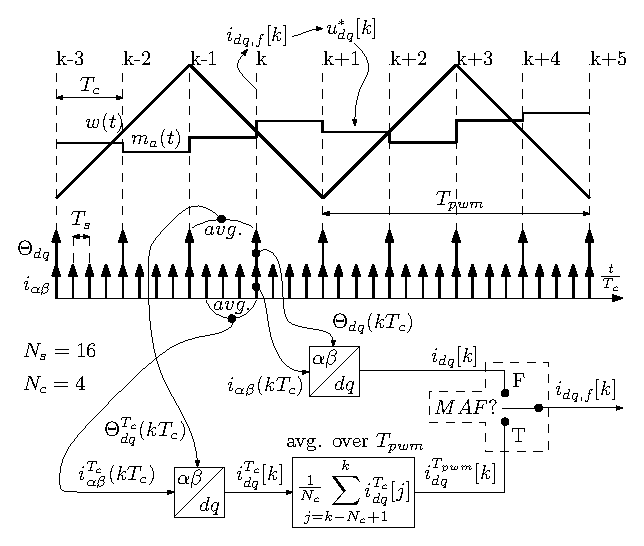
\includegraphics[width=0.95\linewidth]{figures/timing_diagram.eps}}
    \caption{nothing yet}
    \label{fig:timings}
\end{figure}

In case of DS-DU-PWM method, $N_c = N_s = 2$, and only latest values of angle and current signals are used for coordinate-frame transformation to obtain $i_{dq,f}[k]$. This is the standard control method, most-often used in the state-of-the-art digital current controllers []. 

In case of MS-DU-PWM methods, $N_c = 2$, $N_s>2$. This kind of feedback acquisition is analyzed in []. The factor $N_s$ is chosen to be as high as allowed by the maximal ADC sampling rate. At each control interrupt, package of $\alpha \beta$ frame currents is obtained via a DMA buffer, and averaged over $T_c$. This averaged current $\overline{i}_{\alpha \beta}[k]$ is transformed to $dq$ frame using average value of two latest values of $\Theta_{dq}$. In the end, the resulting $dq$ frame current is averaged with the result from the previous interrupt, obtaining the averaged $dq$ current over the time frame of $T_{pwm}$, $\overline{i}_{dq}[k]$. This MAF function is used to obtain the true average value, without the switching ripple component. 

Finally, for the case of MS-MU-PWM methods, the procedure is the same as for MS-DU-PWM methods, except that $N_s \geq N_c > 2$. For MS-MU-PWM methods, MAF can be used in the same manner as for MS-DU-PWM, in order to avoid introducing switching ripple into the control loop. Note that this is not always used, when highest dynamic performance is a goal []. However, for three-phase industrial drives, the effect of nonlinearities introduced by the modulating waveform discontinuities still needs to be investigated. 

For the purpose of later controller tuning, multi-rate system should be analyzed in a unique discrete-time domain, corresponding to the frequency $f_c$. The MAF action is performed at frequency $f_s$, before decimating to $f_c$. For this purpose, to avoid modified $\mathcal{Z}$ transform, MAF can be very closely analyzed using the following transfer function:

\begin{equation}
\begin{aligned}
G_{MAF}(z) = \frac{1 + 2z^{-\frac{N_c}{2}} + z^{-N_c}}{4}.
\label{eq:MAF} 
\end{aligned}    
\end{equation}


\subsection{Total time delay in DSP application}

The discrete-time small-signal model in Fig. \ref{fig:SmallSignal}, all delays are taken into account during the model derivation. 
However, for control loop analysis and comparison between DS-DU, MS-DU, AND MS-MU PWM, based on the crossover frequency and phase margin it is of interest to analyze these delays in continuous-time domain.

The time delay calculation and DPWM modulation is shown in \ref{eq:tauD}. For DS-DU-PWM which doesn't require any feedback filtering, this is equal to the total delay introduced by the control:

\begin{equation}
\begin{aligned}
\tau_{d,DS-DU} = \frac{3}{2} \frac{T_{pwm}}{2}.
\label{eq:tauDSDU} 
\end{aligned}    
\end{equation}

For MS-DU-PWM, MAF is most often used [] to filter out the switching frequency component. The phase lag of the MAF over $T_{pwm}$ can be closely approximated by a pure delay equal to $\frac{T_{pwm}}{2}$ []. This results in the total equivalent time-delay equal to:

\begin{equation}
\begin{aligned}
\tau_{d,MS-DU,MAF} = \frac{3}{2} \frac{T_{pwm}}{2} + \frac{T_{pwm}}{2} = \frac{5}{4} T_{pwm}.
\label{eq:tauMSDU} 
\end{aligned}    
\end{equation}

For MS-MU-PWM without MAF, equivalent time-delay is equal to:

\begin{equation}
\begin{aligned}
\tau_{d,MS-MU} = \frac{3}{2} \frac{T_{pwm}}{N_c}.
\label{eq:tauMSMU} 
\end{aligned}    
\end{equation}

Finally, for MS-MU-PWM with MAF, equivalent time-delay is equal to:
\begin{equation}
\begin{aligned}
\tau_{d,MS-MU,MAF} = \frac{3}{2} \frac{T_{pwm}}{N_c} + \frac{T_{pwm}}{2} = \frac{\frac{3}{N_c}+1}{2}T_{pwm}.
\label{eq:tauMSMUMAF} 
\end{aligned}    
\end{equation}

From above the following can be concluded. First of all, MS-DU-PWM features significant time-delay due to MAF and high modulating and control delays. This kind of feedback acquisition is indeed often necessary due to high deterioration of the signal quality in industrial drives []. However, for high dynamic performance, controller strategy needs to include additional derivative gain compared to \eqref{eq:Controller}. Regarding dynamics, best case represents MS-MU-PWM without MAF. With high multi-update factors $N_c \geq 8$ [], control delays are practically removed and dynamic capabilities approach analog control. This means that the achievable bandwidths are limited purely by PWM frequency. However, strong nonlinearities may exhibit due to the introduction of the switching ripple component 
Finally, from \eqref{eq:tauMSMUMAF} it can be seen that starting from $N_c>6$, equivalent time delay is reduced compared to DS-DU-PWM. This is important, as the same kind of filtering as in MS-DU-PWM is used, which results in a high quality feedback signal in terms of noise content, while the dynamics is improved compared to traditionally used DS-DU-PWM. By filtering the switching ripple, high nonlinearities due to multi-update control are strongly attenuated. 
In the end, it should be mentioned that multi-update control always features additional nonlinear advantage compared to DU, as duty-cycle can be modified $N_c$ times per PWM period, which improves large-signal response of the controller. 


\section{Simulation results}

In order to illustrate benefits of the proposed MS-PWM methodology, three different control loop architectures are examined in this section and their performance is evaluated by means of computer simulations in MATLAB/Simulink.  It is distinguished between different MS-PWM control loop architectures based on current controller structure (IMC with or without differential compensator) and feedback acquisition (with or without MAF). For each architecture of interest, at first, an appropriate benchmark controller is determined. Then, parameter setting procedure for the proposed MS-PWM controllers is explained. Finally, a comparison between proposed and benchmark controllers is illustrated by performance evaluation of the simulated step responses and open-loop frequency response analyses. In addition to this, analytically obtained results are compared with those from simulation, with the aim of verifying modelling approach explained in Section III. \par
Simulation is organized as follows. Current controller is modelled in discrete domain whereas all relevant delays are taken into account. Detailed model of DPWM, which resembles action qualifier module realization within DSP EPWM peripheral, is implemented.  Load is modeled in continuous time domain using Simulink abc machine model. Simulation is developed so that it is easily adjustable for different update rates, controller structures and feedback acquisition paths. Simulation results presented in this section are obtained with BLDC motor from \cite{vuksa2016}.  Switching frequency is set to 10kHz. For the proposed MS-PWM controllers, update rate is set to eight, i.e. acquiring the control variables and updating the modulating waveform is done eight times per switching period. MAF, when used for the feedback acquisition, assumes averaging of 16 samples per switching period. \par
The same simulation model is used to simulate step responses and perform FRA. However, the presented step responses are obtained with $1\mu s$ dead-time, whereas dead-time is set to $0$ when running FRA simulations, so that non-linear effects which could mask FRA responses are avoided. Step responses are obtained at 270Hz electrical frequency. Open loop FRA simulations are organized in the following manner. For the analyzed axis, sinusoidal perturbation of 0.1 A is used as an excitation signal. Error in the other axis is set to zero. The perturbation frequencies are an arithmetic sequence starting from 400 Hz to 5000 Hz, with a step of 50 Hz.\par

\subsection{Control loop architecture 1: N=8 with MAF, IMC}
MS-PWM control loop architecture analyzed in this subsection (further on denoted as C1) assumes IMC controller from \cite{vuksa2016} with MAF in the feedback path. The benchmark for this case (further on denoted as B1) is the state-of-the art double update rate controller with the same IMC and standard synchronous sampling based feedback acquisition, with IMC gain $\alpha$ set to the highest value which results in the response without an overshoot \cite{vuksa2016}. The main advantage of C1, compared to B1, is a considerably enhanced noise suppression capability and a slightly improved dynamic response. IMC gain for C1 is set analytically so that the same cross-over frequency is obtained as for B1. Parameters for B1 and C1 are shown in Table \ref{tab: case 1}. Results presented within this subsection are denoted as test case 1 results. \par


\begin{table}[h!]
			  \caption{Parameters of controllers C1 and B1}
              \label{tab: case 1}
              \centering
              \begin{tabular}{lll}
                           \midrule\midrule
        C1 parameters     & label           & value\\
        \midrule               
                  Update rate   	& $N$      & 8\\  
                  IMC gain    & $\alpha$      & 0.0636    \\
                  Feedback acquisition    & $/$      & MAF\\
                  \midrule\midrule
        B1 parameters & label           & value\\
                  \midrule
                  Update rate   	& $N$      & 2\\  
                  IMC gain    & $\alpha$      & 0.25    \\
                  Feedback acquisition    & $/$      & sync. sampl.\\                                                         
                  \midrule\midrule
              \end{tabular}
\end{table}

Q current step responses for C1 and B1 are shown in Fig. \ref{fig:C1_step}-\ref{fig:B1_step}. Presented waveforms are dq currents obtained by sampling and transformation process described in Section II. Acc. to the results in Fig. \ref{fig:C1_step} no coupling between axes is present. Even though step response itself is insufficient to fully describe dynamic behaviour of the control loop, it might be useful to get an insight and a rough estimate of the controller performance. Simulated and analytical step response characteristics for C1 and B1 are listed in Table \ref{tab:C1_step}. Note that analytical rise time is calculated as $\pi/(10*f_{bw-3dB}^{an})$. According to the results in Table \ref{tab:C1_step}, C1 offers slightly improved dynamic performance compared to B1, which is expected, taking into account parameter setting procedure for the proposed controller. A slight mismatch between analytically calculated and simulated rise times both for C1 and B1, might be a consequence of the unmodelled dead-time non-linearities and an approximation used when deriving a feedback averaging model. \par

\begin{figure}[t!]
    \centerline{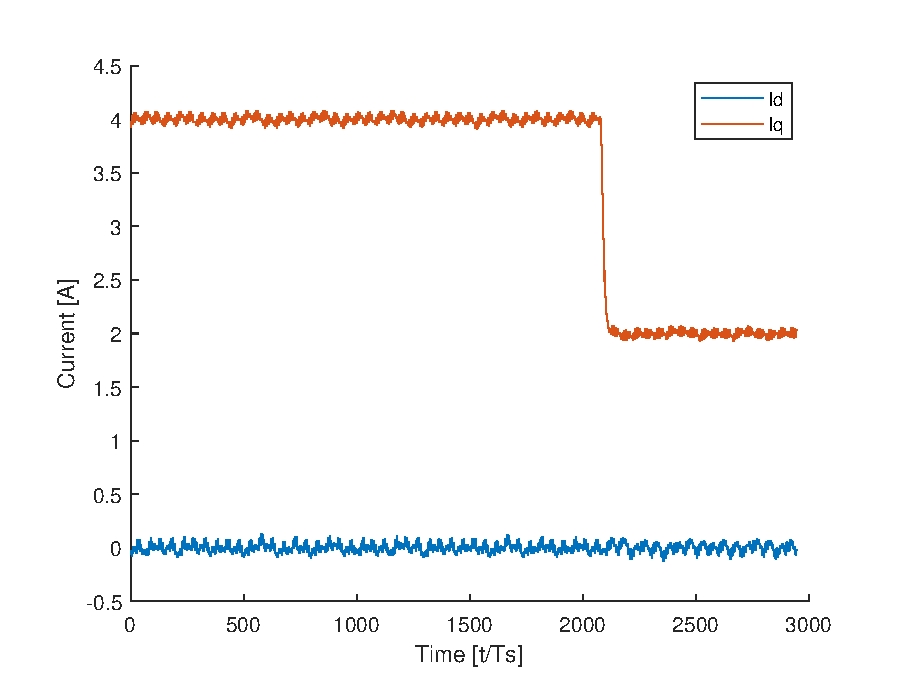
\includegraphics[width=0.95\linewidth]{figures/C1_step.eps}}
    \caption{Simulated step response for C1.}
    \label{fig:C1_step} 
\end{figure}

\begin{figure}[t!]
    \centerline{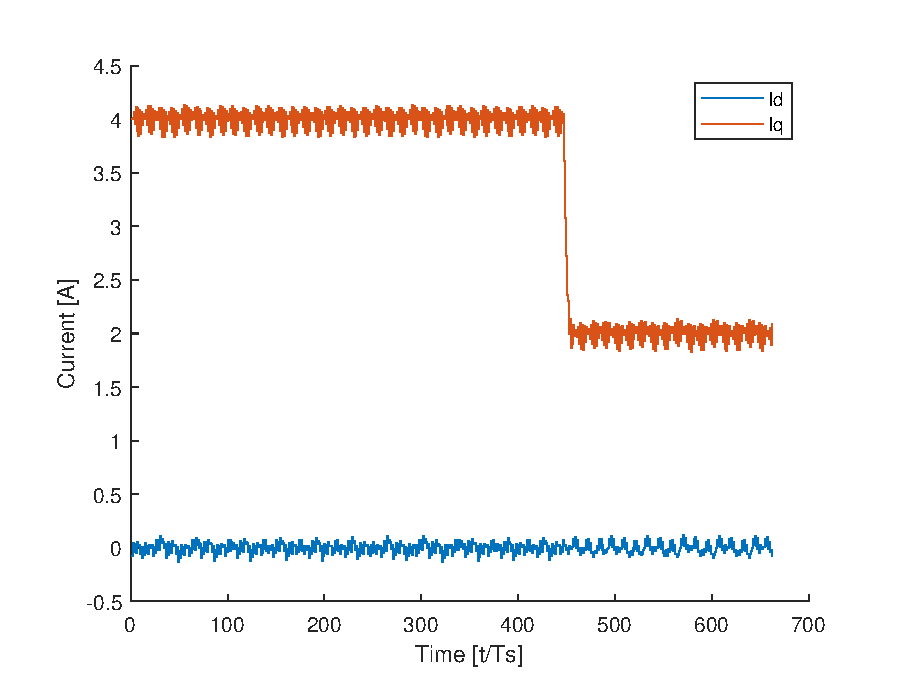
\includegraphics[width=0.95\linewidth]{figures/B1_step.eps}}
    \caption{Simulated step response for B1.}
    \label{fig:B1_step} 
\end{figure}

\begin{table}[h!]
			  \caption{Simulated step response characteristics for test case 1}
              \label{tab:C1_step}
              \centering
              \begin{tabular}{llll}
                           \midrule\midrule
        C1 characteristics & label & value   & unit\\
        \midrule               
                  Analytical 3dB closed loop bandwidth	& $f_{bw-3dB}^{an}$ & 1.3871 &kHz\\  
                  Analytical rise time  & $t_{rise}^{an}/T{pwm}$ & 2.2685 & /   \\
                  Simulated rise time  & $t_{rise}^{sim}/T{pwm}$ & 2.75 & /   \\
                  \midrule\midrule
        B1 characteristics & label           & value    & unit\\
                  \midrule
                  Analytical 3dB closed loop bandwidth	& $f_{bw-3dB}^{an}$ & 1.4607 &kHz\\  
                  Analytical rise time  & $t_{rise}^{an}/T{pwm}$ & 2.1542 & /   \\
                  Simulated rise time  & $t_{rise}^{sim}/T{pwm}$ & 2.4 & /   \\
                  \midrule\midrule
                                                        
              \end{tabular}
\end{table}

Q axis open loop FRA results for test case 1 are shown in Fig. \ref{fig:tc1_olfra}.  Comparison between simulated and analytical C1 FRA performance, as well as analytical B1 performance are listed in Table \ref{tab:tc1_olfra}. These results validate derived MS-PWM control loop analytical model, since mismatch between analytical and simulated C1 waveforms is hardly noticeable and exists only in the higher frequency range. In addition to this, cross-over frequency and phase margin of the simulated C1 control loop are similar to those of B1, which is in agreement with the parameter setting procedure described above. Therefore, test case 1 illustrates that MS-PWM approach offers MAF based feedback acquisition without degrading control loop dynamic performance. In this way, the noise and sampling errors in the feedback path are successfully eliminated due to MAF based feedback acquisition, but also the dynamic performance is kept high. \par

\begin{figure}[t!]
    \centerline{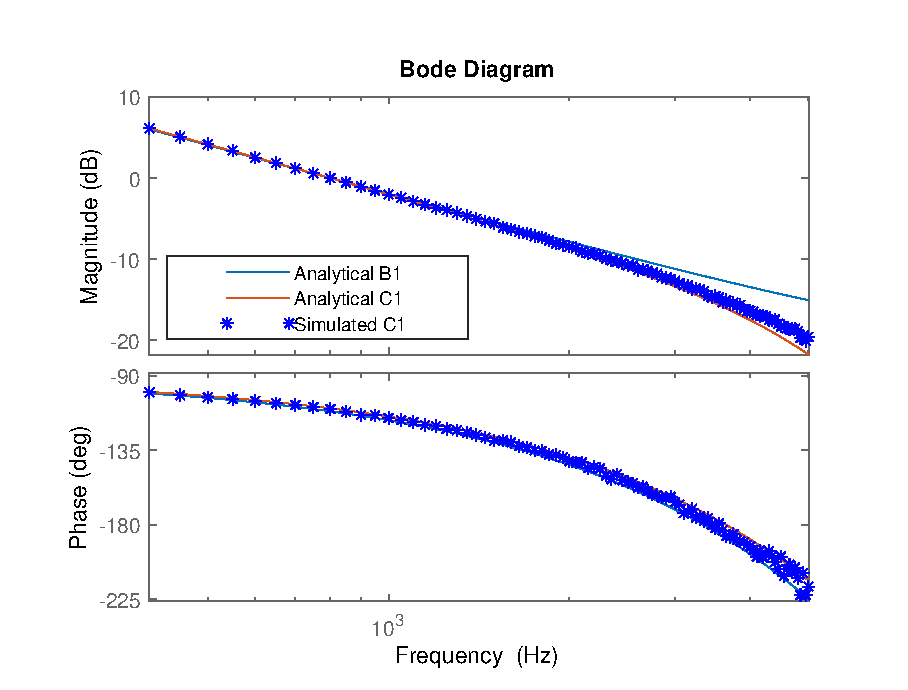
\includegraphics[width=0.95\linewidth]{figures/tc1_olfra.eps}}
    \caption{Simulated open loop FRA for test case 1.}
    \label{fig:tc1_olfra} 
\end{figure}

\begin{table}[h!]
			  \caption{Open loop FRA performance for test case 1}
              \label{tab:tc1_olfra}
              \centering
              \begin{tabular}{llll}
                           \midrule\midrule
        C1 characteristics & label & value   & unit\\
        \midrule               
                  Analytical cross-over frequency	& $f_{c}^{an}$ & 798.5845 &Hz\\
                  Simulated cross-over frequency	& $f_{c}^{sim}$ & 800 &Hz\\ 
                  Analytical phase margin  & $pm^{an}$ & 70.2667 &  $^\circ$   \\
                  Simulated phase margin  & $pm^{sim}$ & 70 &  $^\circ$   \\
                  \midrule\midrule
                  B1 characteristics & label  & value    & unit\\
                  \midrule
                  Analytical cross-over frequency	& $f_{c}^{an}$ & 799.1594 &Hz\\
                  Analytical phase margin  & $pm^{an}$ & 68.4572 &  $^\circ$   \\
                  \midrule\midrule
                                                        
              \end{tabular}
\end{table}

\subsection{Control loop architecture C2: N=8 with MAF, IMC + dif.}
MS-PWM control loop architecture analyzed in this subsection (further on denoted as C2) assumes IMC controller with differential compensator from \cite{vuksa2017} and MAF in the feedback path. This  case  is  given  to demonstrate  that  MS-PWM  can  offer  even  better  dynamics than  reported  in \cite{vuksa2017}. The benchmark for this case (further on denoted as B2) assumes controller structure proposed in \cite{vuksa2017} - double update rate IMC controller with improved performance indices, differential compensator and MAF based feedback acquisition. In simulations, the advanced scheduling scheme for B2 is implemented without neglecting execution time so that the results are suitable for comparison with standard code implementation which does not assume execution time optimization. Gains for IMC and differential compensator in case of B2 are set to the optimal values from \cite{vuksa2017}. Parameter setting procedure used for C2 is similar to the one proposed in \cite{vuksa2017}. Parameters for B2 and C2 are shown in Table \ref{tab: case 2}. Results presented within this subsection are denoted as test case 2 results. 
\par

\begin{table}[h!]
			  \caption{Parameters for controllers C2 and B2}
              \label{tab: case 2}
              \centering
              \begin{tabular}{lll}
                           \midrule\midrule
        C2 parameters     & label           & value\\
        \midrule               
                  Update rate   	& $N$      & 8\\  
                  IMC gain    & $\alpha$      & 0.12038    \\
                  Differential gain    & $d$      & 2.1948    \\
                  Feedback acquisition    & $/$      & MAF\\
                  \midrule\midrule
        B2 parameters & label           & value\\
                  \midrule
                  Update rate   	& $N$      & 2\\  
                  IMC gain    & $\alpha$      & 0.38    \\
                  Differential gain    & $d$      & 0.444    \\
                  Feedback acquisition    & $/$      & MAF\\                                                         
                  \midrule\midrule
              \end{tabular}
\end{table}

Q current step responses for C2 and B2 are shown in Fig. \ref{fig:C2_step}-\ref{fig:B2_step}. Presented waveforms are dq currents obtained by sampling and transformation process described in Section II. Oscillations at the fundamental frequency are visible in C2 step response (Fig. \ref{fig:C2_step_sub1}). Poor disturbance rejection capability due to small phase resistance might be the root cause of these oscillations, since with 5 times larger stator phase resistance oscillations are not present (Fig. \ref{fig:C2_step_sub2}). In Fig. \ref{fig:B2_step}, two different step responses are shown to illustrate that oscillations at the fundamental frequency exist in the benchmark response too, but are of smaller amplitude and present only in case step reference change is larger.  Source of the aforementioned oscillations needs to examined in more detail and will be considered as part of the future work. Addition of an active resistance feedback  could be considered \cite{vuksa2018} if insufficient disturbance rejection capability of the proposed MS-PWM controller proves to be an issue.\par
Simulated and analytical step response characteristics for C1 and B1 are listed in Table \ref{tab:C2_step}. Note that analytical transfer function for B2 assumed zero delay i.e. neglected execution time as in \cite{vuksa2017}, since analytical representation of execution time which is smaller than regulation period would require modified Z transform. According to the results in Table \ref{tab:C2_step}, C2 offers better dynamic performance than B2. \par

\begin{figure}[t!]
\centering
\begin{subfigure}{0.5\textwidth}
  \centering
  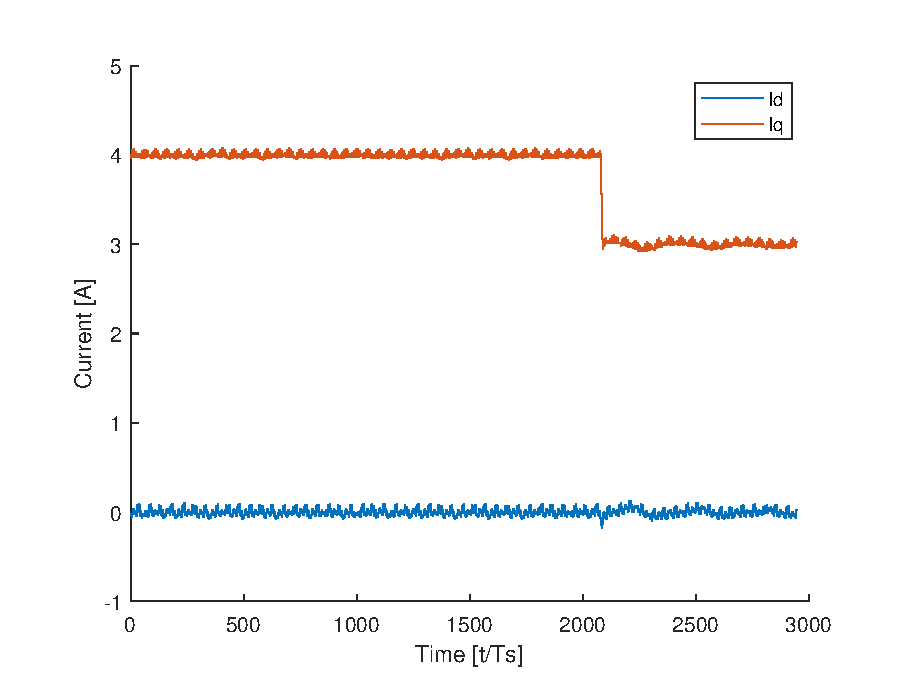
\includegraphics[width=0.95\linewidth, height = 45mm]{figures/C2_step.eps}
  \caption{}
  \label{fig:C2_step_sub1}
\end{subfigure}\\
\begin{subfigure}{0.5\textwidth}
  \centering
  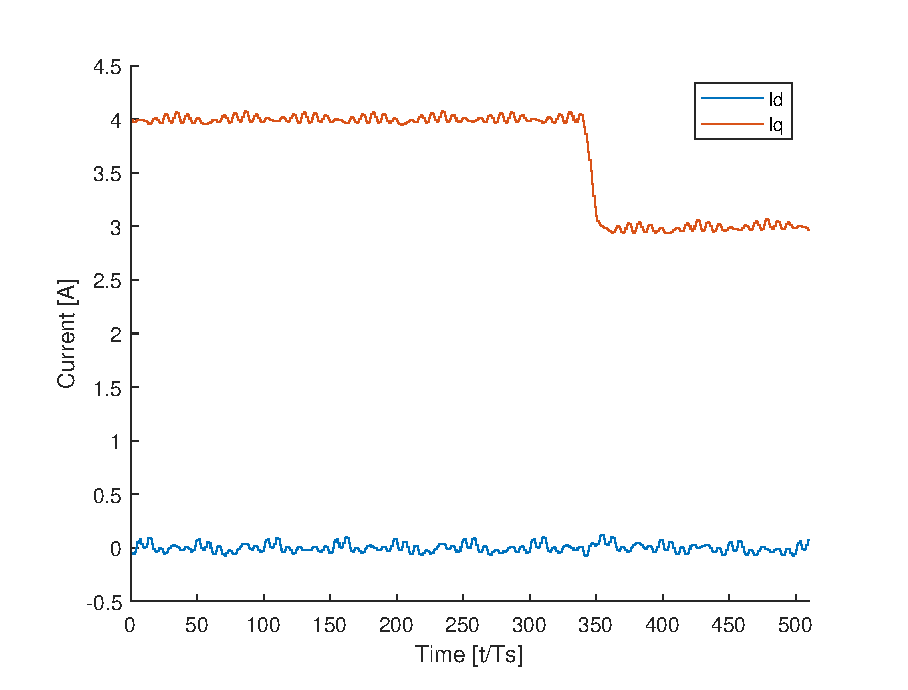
\includegraphics[width=0.95\linewidth, height = 45mm]{figures/C2_step_5Rs.eps}
  \caption{}
  \label{fig:C2_step_sub2}
\end{subfigure}\\
\caption{Simulated step response for C2: (a) original phase resistance; (b) 5 times larger phase resistance.}
\label{fig:C2_step}
\end{figure}

\begin{figure}[t!]
    \centerline{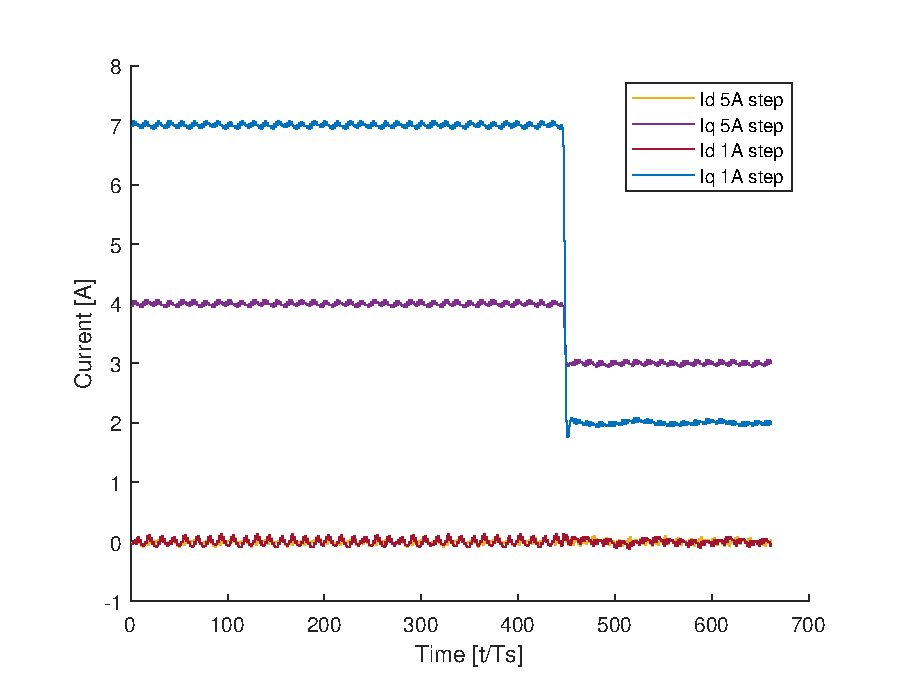
\includegraphics[width=0.95\linewidth]{figures/B2_step.eps}}
    \caption{Simulated step response for B2.}
    \label{fig:B2_step} 
\end{figure}

\begin{table}[h!]
			  \caption{Simulated step response characteristics for test case 2}
              \label{tab:C2_step}
              \centering
              \begin{tabular}{llll}
                           \midrule\midrule
        C2 characteristics & label & value   & unit\\
        \midrule               
                  Analytical 3dB closed loop bandwidth	& $f_{bw-3dB}^{an}$ & 3.9846
  &kHz\\  
                  Analytical rise time  & $t_{rise}^{an}/T{pwm}$ & 0.7897 & /   \\
                  Simulated rise time  & $t_{rise}^{sim}/T{pwm}$ & 1.125 & /   \\
                  \midrule\midrule
        B2 characteristics & label & value    & unit\\
                  \midrule
                  Analytical 3dB closed loop bandwidth	& $f_{bw-3dB}^{an}$ & 3.5105 &kHz\\  
                  Analytical rise time  & $t_{rise}^{an}/T{pwm}$ & 0.8964  & /   \\
                  Simulated rise time  & $t_{rise}^{sim}/T{pwm}$ & 1.25 & /   \\
                  \midrule\midrule
                                                        
              \end{tabular}
\end{table}

Q axis open loop FRA results for test case 2 are shown in Fig. \ref{fig:tc2_olfra}.  Comparison between simulated and analytical C2 FRA performance, as well as analytical B2 performance are listed in Table \ref{tab:tc2_olfra}. Analytical and simulated waveforms for C2 are in good agreement, despite in the high frequency range  where the MS-PWM control loop modelling approach described in Section II is of lower precision. C2 results in $1.5kHz$ cross-over frequency which is $25\%$ higher than that of B2, whereas phase margin remains around $66^\circ$ for both control loop architectures. Thus, the test case 2 illustrates that the MS-PWM approach offers better dynamic performance than the controller proposed in  \cite{vuksa2017}.\par

\begin{figure}[t!]
    \centerline{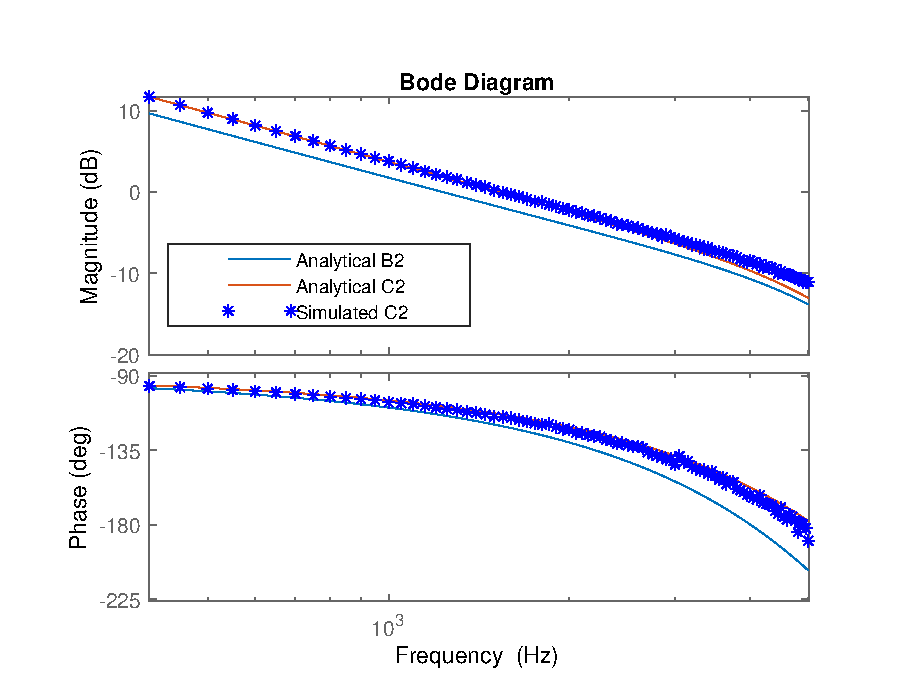
\includegraphics[width=0.95\linewidth]{figures/tc2_olfra.eps}}
    \caption{Simulated open loop FRA  for test case 2.}
    \label{fig:tc2_olfra} 
\end{figure}

\begin{table}[h!]
			  \caption{Open loop FRA performance for test case 2}
              \label{tab:tc2_olfra}
              \centering
              \begin{tabular}{llll}
                           \midrule\midrule
        C2 characteristics & label & value   & unit\\
        \midrule               
                  Analytical cross-over frequency	& $f_{c}^{an}$ & 1.5209 &kHz\\
                  Simulated cross-over frequency	& $f_{c}^{sim}$ & 1.55 &kHz\\ 
                  Analytical phase margin  & $pm^{an}$ & 66.838 &  $^\circ$   \\
                  Simulated phase margin  & $pm^{sim}$ & 65.135 &  $^\circ$   \\
                  \midrule\midrule
                  B2 characteristics & label  & value    & unit\\
                  \midrule
                  Analytical cross-over frequency	& $f_{c}^{an}$ & 1.2283 &kHz\\
                  Analytical phase margin  & $pm^{an}$ & 66.068 &  $^\circ$   \\
                  \midrule\midrule
                                                        
              \end{tabular}
\end{table}

\subsection{Control loop architecture C3: N=8 without MAF, IMC}
MS-PWM control loop architecture analyzed in this subsection (further on denoted as C3) consists of IMC controller without any filters in the feedback. A benchmark for this case is the same as the benchmark for the previously analyzed case. C3
is expected to provide the dynamics better than B2, using discrete IMC
without differential compensator. IMC gain for C3 is set analytically so
that higher -3dB bandwidth is achieved than in case of the benchmark. Parameters for C3 are shown in Table \ref{tab: case 3}. Results presented within this subsection are denoted as test case 3 results. 

\begin{table}[h!]
			  \caption{Parameters for controller C3}
              \label{tab: case 3}
              \centering
              \begin{tabular}{lll}
                           \midrule\midrule
        C3 parameters     & label           & value\\
        \midrule               
                  Update rate   	& $N$      & 8\\  
                  IMC gain    & $\alpha$      & 0.2    \\
                  Feedback acquisition    & $/$      & no filters\\
                  \midrule\midrule

              \end{tabular}
\end{table}
Q current step response for C3 is shown in Fig. \ref{fig:C3_step}. Presented waveforms are obtained by taking each 4th sample of the dq currents which are result of the sampling and transformation process described in Section II. The aim of such a representation is to avoid plotting switching ripple which, in case of C3, is present in the sampled dq currents, so that the results are comparable with previously presented ones. In this way, represented waveforms are equivalent, in terms of switching ripple magnitude, as those obtained by conventional double update synchronous sampling. Note that no coupling between axis is present in Fig. \ref{fig:C3_step}. Simulated and analytical C3 step response characteristics are listed in Table \ref{tab:C3_step}. According to the results in Table \ref{tab:C2_step} and \ref{tab:C3_step}, C3 offers slightly improved dynamics compared to B2. Further increase of IMC gain for C3 could theoretically result in even faster step response. However, practical implementation aspects of the higher gains without any filters in the feedback have to be carefully examined. 

\begin{figure}[t!]
    \centerline{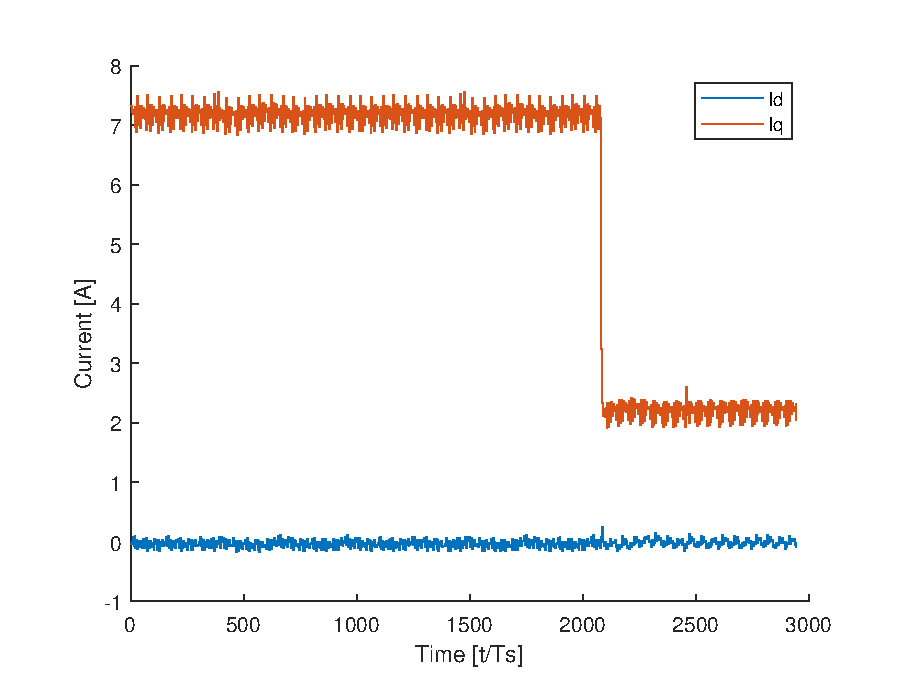
\includegraphics[width=0.95\linewidth]{figures/C3_step.eps}}
    \caption{Simulated step response for C3.}
    \label{fig:C3_step} 
\end{figure}

\begin{table}[h!]
			  \caption{Simulated step response characteristics for test case 3}
              \label{tab:C3_step}
              \centering
              \begin{tabular}{llll}
                           \midrule\midrule
        C3 characteristics & label & value   & unit\\
        \midrule               
                  Analytical 3dB closed loop bandwidth	& $f_{bw-3dB}^{an}$ & 3.9467
  &kHz\\  
                  Analytical rise time  & $t_{rise}^{an}/T{pwm}$ & 0.7973 & /   \\
                  Simulated rise time  & $t_{rise}^{sim}/T{pwm}$ & 0.8594 & /   \\
                  \midrule\midrule
                                                        
              \end{tabular}
\end{table}

Q axis open loop FRA results for test case 3 are shown in Fig. \ref{fig:tc3_olfra}. Magnitude of the analytical and simulated waveforms for C3 are in good agreement. Simulated C3 phase characteristic, however, is slightly lower the analytical one. Comparison between simulated and analytical C3 FRA performance, as well as analytical B2 performance are listed in Table \ref{tab:tc3_olfra}. According to the results in Table \ref{tab:tc2_olfra} and \ref{tab:tc3_olfra}, C3 offers considerably higher cross-over frequency than B2, whereas phase margin remains the same. Practical implementation of C3 might require addition of a low-pass filter in the feedback path in order to avoid issues which might arise as a consequence of sampling the switching noise. For $N=8$, this is especially pronounced in the vicinity of the duty cycles which are equal to $0.25, 0.5$ and $0.75$ ref?.\par

\begin{figure}[t!]
    \centerline{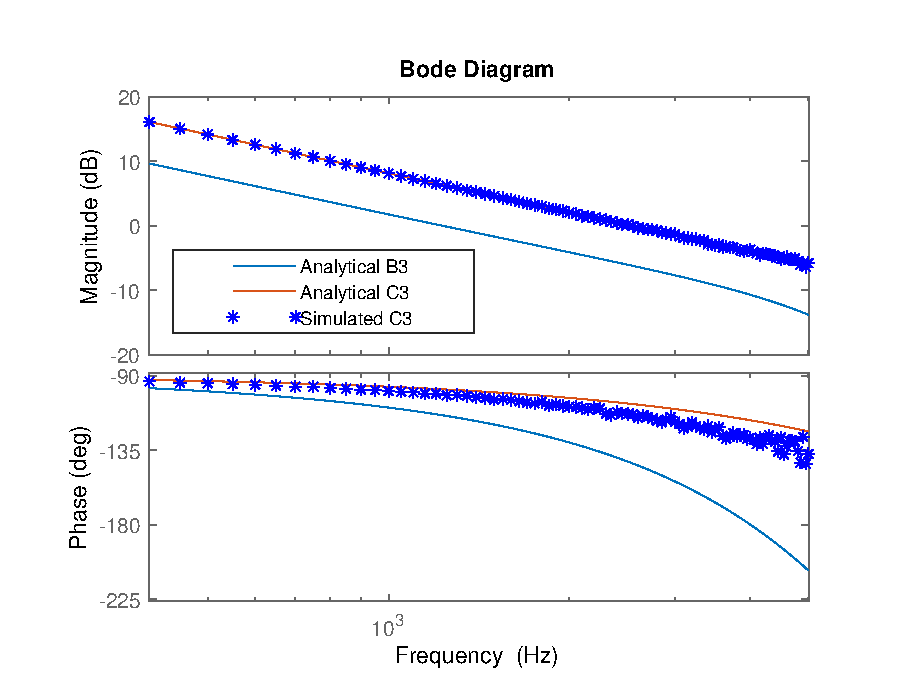
\includegraphics[width=0.95\linewidth]{figures/tc3_olfra.eps}}
    \caption{Simulated open loop FRA  for test case 3.}
    \label{fig:tc3_olfra} 
\end{figure}

\begin{table}[h!]
			  \caption{Open loop FRA performance for test case 3}
              \label{tab:tc3_olfra}
              \centering
              \begin{tabular}{llll}
                           \midrule\midrule
        C3 characteristics & label & value   & unit\\
        \midrule               
                  Analytical cross-over frequency	& $f_{c}^{an}$ & 2.5548 &kHz\\
                  Simulated cross-over frequency	& $f_{c}^{sim}$ & 2.55 &kHz\\ 
                  Analytical phase margin  & $pm^{an}$ & 72.7824 &  $^\circ$   \\
                  Simulated phase margin  & $pm^{sim}$ & 66.5165 &  $^\circ$   \\
                  \midrule\midrule
                                                        
              \end{tabular}
\end{table}

\section{Experimental verification}

\section{Conclusion}


\ifCLASSOPTIONcaptionsoff
  \newpage
\fi

\bibliographystyle{IEEEtran}
% argument is your BibTeX string definitions and bibliography database(s)
\bibliography{IEEEabrv,bib/mybibliography.bib}

\end{document}



